\documentclass[9pt]{beamer}
\mode<presentation>
\usepackage[T1]{fontenc}
\usepackage{color}
\usepackage{graphicx}
\usepackage{natbib}
\usepackage{tikz}
\usetikzlibrary{shapes.geometric}
\usepackage{xmpmulti}
\usepackage{animate}
\usepackage{tcolorbox}
\usepackage{amsmath}
\usepackage{gensymb}
\usepackage{csquotes}
\usepackage{bibentry}
\nobibliography*

%\usetheme{Singapore}

\setbeamercolor{block title}{bg=structure!20}
\setbeamercolor{block body}{bg=structure!10}
\setbeamertemplate{blocks}[rounded][shadow]
%\usecolortheme{seahorse}

\usefonttheme{professionalfonts}

\title[Climate Impacts]{Scaling up assessments of regional impacts of climate change: a rapid, computer-assisted systematic map}
\author{Max Callaghan, Jan Minx, Carl-Friedrich Schleussner, Gerrit Hansen, Quentin Lejeune, Shruti Nath, Emily Theokritoff, Marina Andrijevic, Robert Brecha, Michael Hegarty, Chelsea Jones, Kaylin Lee, Agathe Lucas, Nicole van Maanen, Inga Menke, Peter Pfleiderer, Burcu Yesil }
\institute[MCC]{
	\includegraphics[height=1cm,width=2cm]{images/MCC_Logo_RZ_rgb.jpg} \hspace{5em} \includegraphics[height=1cm]{images/climate_analytics.png}
}

\newif\ifframeinlbf
\frameinlbftrue
\makeatletter
\newcommand\listofframes{\@starttoc{lbf}}
\makeatother

\addtobeamertemplate{frametitle}{}{%
	\ifframeinlbf
	\addcontentsline{lbf}{section}{\protect\makebox[2em][l]{%
			\protect\usebeamercolor[fg]{structure}\insertframenumber\hfill}%
		\insertframetitle\par}%
	\else\fi
}

\newtheorem*{remark}{}

\bibliographystyle{apalike}

\begin{document}
	
\begin{frame}
	\titlepage
\end{frame}


%%%%%%%%%%%%%%%%%%%%%%%%%%%%%%%%%%%%%%%%%%%%%%%%%%
%% Introduction
\section{Introduction}

%\begin{frame}
%\tableofcontents[currentsection]
%\end{frame}

\begin{frame}{Context}

Systematic assessments of the evidence on Climate Change like those conducted by the IPCC are vital.

\begin{columns}
	\begin{column}{0.618\linewidth}
		\begin{figure}
			\includegraphics[width=\linewidth]{../map_18.png}<1->
		\end{figure}
	\end{column}
	\begin{column}{0.312\linewidth}
		
		\begin{figure}
			\includegraphics[width=\linewidth]{images/pubs_time_wgb_lp.pdf}<2->
		\end{figure}
		
		\begin{itemize}
			\small
			\item<2->These are challenged by big literature \cite{Callaghan2020} 
			\item<3->They do not account for uncertainty about what literature is available
		\end{itemize}
	\end{column}
\end{columns}

\end{frame}

%\begin{frame}{Quantifying the literature}
%
%\begin{columns}
%	
%	\begin{column}{0.382\linewidth}
%	\begin{itemize}
%		\item AR5 WGII started with a basic bibliometric analysis of climate change (and impacts and adaptation) literature
%		\item The literature has doubled again since then
%		\item We can do more than this
%	\end{itemize}
%\end{column}
%
%	\begin{column}{0.618\linewidth}
%		\begin{figure}
%			\includegraphics[width=0.7\textheight]{ar5_fig_1_1}
%		\end{figure}
%	\end{column}
%
%\end{columns}
%
%\end{frame}


\begin{frame}{Process}

\begin{enumerate}
	\item Broad \textbf{search} in literature databases (Web of Science \& Scopus) for literature on climate impacts
	\item Hand \textbf{screen and code} documents to include only documents on observed climate impacts, and code the type of impacts and type of evidence
	\item Combine this training data with the categorisation of documents in \textbf{AR5}
	\item Use supervised \textbf{machine learning} to predict the inclusion and impact type of 100s of thousands or remaining documents
	\item Use named entity recognition to extract \textbf{geographical locations} from titles and abstracts
	\item Map entities to grid cells and combine with \textbf{WGI style D\&A} of temperature and precipitation trends at the grid cell level
	\item Describe \textbf{evidence gluts and gaps} at a grid cell level
	
\end{enumerate}

\end{frame}

\begin{frame}{We set up our platform to record the relevance and lots of other information about each document}

\begin{figure}
	\includegraphics[width=\linewidth]{../plots/screening-platform}
\end{figure}

\end{frame}

%%%%%%%%%%%%%%%%%%%%%%%%%%%%%%%%%%%%%%%%%%%%%%%%%%
%% Machine learning
\section{Machine learning}

%\begin{frame}
%\tableofcontents[currentsection]
%\end{frame}

\begin{frame}{Feature space - text as data}

The set of features is a TFIDF weighted set of unigrams and bigrams from the documents' abstracts

\medskip

\begin{columns}
	\begin{column}{0.5\linewidth}
		\includegraphics[width=\linewidth]{images/doc_example.png}
	\end{column}
	\begin{column}{0.5\linewidth}
		\includegraphics[width=\linewidth]{images/example_doc_tfidf.pdf}
	\end{column}
\end{columns}

\medskip

We discard very uncommon and very common features, leaving us with a vocabulary of 7,394 unique features.

\end{frame}

\begin{frame}{Setup}
We need two types of classifiers:
\begin{itemize}
	\item A binary, include/don't include classifier
	\item Various multilabel classifiers for impact types, attribution categories and climate drivers
\end{itemize}

\begin{columns}
	\begin{column}{0.618\linewidth}
		\begin{figure}
			\includegraphics[width=\linewidth]{images/svc_sklearn_unbalanced.png}
		\end{figure}
	\end{column}
	\begin{column}{0.382\linewidth}
		We use Support Vector Machines (SVMs), which draw hyperplanes through the feature space which best separate the classes
		
		\bigskip
		
		Note that a state of the art language model such as BERT may outperform SVMs, but these are resource and data hungry, and less transparent
	\end{column}
\end{columns}

\end{frame}



%\begin{frame}{We predict tens of thousands of additional documents relevant according to the criteria we defined}
%
%\begin{columns}
%	\begin{column}{0.618\linewidth}
%		\begin{figure}
%			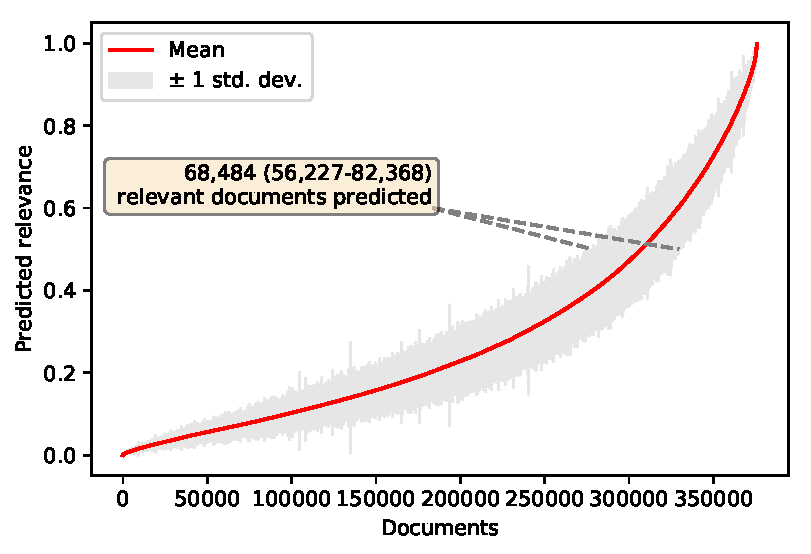
\includegraphics[width=\linewidth]{../plots/prediction_models/predictions_unseen.png}
%		\end{figure}
%	\end{column}
%	\begin{column}{0.382\linewidth}
%		\begin{itemize}
%			\item We train 10 classifiers on random partitions of the labelled dataset
%			\item This gives us 10 estimates for each unseen document
%			\item The mean and standard deviation of these estimates give us an idea, with some uncertainty, of how many documents are in each category
%		\end{itemize}
%	\end{column}
%\end{columns}
%
%\end{frame}

\begin{frame}{Results}

\begin{columns}
	\begin{column}{0.618\linewidth}
		\begin{figure}
			\includegraphics[width=\linewidth]{../figures/figure_1_CFS.png}
		\end{figure}
	\end{column}
	\begin{column}{0.382\linewidth}
		\begin{itemize}
			\item We identify nearly 100,000 documents likely to be relevant
			\item We can predict impact type, attribution type, and location
		\end{itemize}
	
		From here we focus on ``Trend attribution'' documents, that is, documents attributing impacts to a trend in a climate variable, and specifically focus on trends driven by temperature and precipitation
	\end{column}
\end{columns}



\end{frame}

%%%%%%%%%%%%%%%%%%%%%%%%%%%%%%%%%%%%%%%%%%%%%%
%% D&A


\begin{frame}{Synthesizing impacts evidence with quantitative detection and attribution evidence}

We know from detection and attribution studies whether observed trends in temperature and precipitation are attributable to human influence on the climate.

\cite{Knutson2013, Knutson2018} show this on a grid cell level

\begin{columns}
	\begin{column}{0.65\linewidth}
		\includegraphics[width=\linewidth]{images/knutson_precip_da}
	\end{column}
	\begin{column}{0.35\linewidth}
		\includegraphics[width=\linewidth]{images/knutson_temp_da}
	\end{column}
\end{columns}

We can combine this with information from our database of impacts evidence, in which the locations, and the climate drivers have been predicted

\end{frame}

\begin{frame}{Synthesising impacts with D\&A evidence}
\begin{columns}
	\begin{column}{0.4\linewidth}
		\includegraphics[width=\linewidth]{../plots/maps/sudan_precipitation.png}
	\end{column}

	\begin{column}{0.4\linewidth}
		\includegraphics[width=\linewidth]{../plots/maps/sudan_gridcell_count.png}
	\end{column}
\end{columns}

\begin{itemize}
	\item 11 out of 27 gridcells in Sudan contain a reduction in rainfall attributable to human influence on the climate
	\item Each study referring to Sudan (as the smallest identifiable geographical entity)  and predicted to document impacts driven by precipitation refers to a place where around 41\% of the gridcells are known to have anthropogenic changes in precipitation
\end{itemize}
\end{frame}

\begin{frame}{Synthesising impacts with D\&A evidence}
\begin{columns}
\begin{column}{0.4\linewidth}
	\includegraphics[width=\linewidth]{../plots/maps/sudan_precipitation_studies.png}
\end{column}

\begin{column}{0.4\linewidth}
	\includegraphics[width=\linewidth]{../plots/maps/sudan_precipitation_study_places.png}
\end{column}
\end{columns}

\begin{itemize}
\item 7 studies refer to Sudan (as the smallest identifiable geographical entity), and Sudan has 27 gridcells
\item We apportion these studies to the relevant gridcells, calculating that each gridcell in Sudan has $\frac{7}{27}$ studies referring to it
\item We do the same for each further geographical entity
\end{itemize}
\end{frame}

\begin{frame}{We combine all this information to show evidence gaps and gluts}

\begin{columns}
	\begin{column}{1\linewidth}
		\begin{figure}
			\includegraphics[width=\linewidth]{../figures/figure_2_CFS_10_28.png}
		\end{figure}
	\end{column}
%	\begin{column}{0.3\linewidth}
%		 \small
%		\begin{itemize}
%			\item In North America, most studies refer to places and drivers where a minority of gridcells show an attributable trend
%			\item In Africa, the opposite is the case
%		\end{itemize}
%	\end{column}
\end{columns}

\end{frame}

\begin{frame}{Conclusions}

\begin{itemize}
	\item We identify a large body of evidence about climate impacts, including 17,273 studies documenting impacts in areas where we know at least a part of which are changing due to human influence on the climate (11,089 studies where the majority of gridcells show attributable trends)
	\item What we know about the effects of a changing climate on human and natural systems does not always match with what we know about how (and where) humans are driving changes in climate variables 
\end{itemize}

\textbf{But}, 

\begin{itemize}
	\item Current results only show studies in Web of Science, so definitely do not show all relevant studies
	\item Although our query returned all papers in the relevant AR5 section, it may still miss potentially relevant literature.
	\item Study identification is approximate and uncertain, trends in studies may not correspond to trends attributed
	\item Geoparsing is also inexact, and is unable to grasp fuzzy geographical content e.g. "Western China"
	\item In large parts of the world, we do not even know reliably if precipitation and temperature are changing
\end{itemize}

\end{frame}

\begin{frame}{Summary - Scaling up assessments of regional impacts of climate change: a rapid, computer-assisted systematic map}

\begin{columns}
	\small
	\begin{column}{0.5\linewidth}
		\begin{itemize}
			\item In a large collaborative coding exercise, we examined thousands of papers \textit{potentially} relevant to understanding observed impacts of climate change
			\item We used machine learning to identify tens of thousands of studies \textit{likely} to be relevant.
			\item We predicted the sector, climate driver, evidence type and location for each of these studies
			\item We used the location and predicted climate driver to synthesise this information with existing quantitative Detection and Attribution knowledge.
		\end{itemize}
	\end{column}

	\begin{column}{0.5\linewidth}
		
		\begin{block}{Takeaways}
			\begin{itemize}
				\item Machine learning can inform and support global environmental assessments
				\item We have lots of evidence of observed impacts of climate change, including 17,000 studies documenting impacts in areas we know are changing due to human influence on the climate
				\item What we know about the effects of a changing climate on human and natural systems does not always match with what we know about how (and where) humans are driving changes in climate variables 
			\end{itemize}
		\end{block}
		
	\end{column}
\end{columns}



\begin{center}
	\line(1,0){250}
	
	\medskip
	
	\textbf{Thanks!}
	
	\medskip
	
	Contact: \url{callaghan@mcc-berlin.net}

\end{center}



\end{frame}

%%%%%%%%%%%%
%% Bib
\begin{frame}{Bibliography}
\bibliography{../mendeley}
\end{frame}

\end{document}